\documentclass[10pt,a4paper]{article}
\usepackage[utf8]{inputenc}
\usepackage[T1]{fontenc}
\usepackage[margin=2.2cm]{geometry}
\usepackage{booktabs}
\usepackage{graphicx}
\usepackage{array}
\usepackage[expansion=false]{microtype}
\usepackage[numbers,sort&compress]{natbib}
\usepackage[colorlinks=true,linkcolor=black,citecolor=black,urlcolor=black]{hyperref}
\usepackage{enumitem}
\usepackage[font=small,labelfont=bf]{caption}
\setlist{nosep}
\setlength{\emergencystretch}{2em}
\setlength{\tabcolsep}{4.5pt}
\title{Ikhtibar: what public documents require, recommend and describe about testing AI systems before deployment, and how far the evidence can be trusted}
\author{Huda Mueen\\Independent researcher, United Arab Emirates}
\date{}
\begin{document}
\maketitle

\begin{abstract}
Governments, standards bodies and institutes have published many documents that mention testing AI systems before deployment, but the documents differ in force: some require testing, some recommend it and some only describe it. We build an evidence table of 522 provisions from 112 public primary documents in 18 families, coded by binding force and by type of test, and we analyse the 290 test provisions (from 71 documents in 16 families) that pass a verification screen. Binding provisions (mandatory or conditional) are a minority, 28\% of the headline rows, and at most 44.1\% under the most favourable of the alternative assumptions we tried (a bootstrap over documents gives a 95\% interval of 13.4 to 43.7 for the share as coded). Binding provisions are not more specific than the others: in a blind coding of all headline rows they are more often process only (about 24.7\% to 30.9\% against 7.5\% to 11.5\%), and we find no reliable difference in how often they name a method, metric or criterion. The paper's second contribution is a protocol for auditing an evidence table of this kind: baselines show that binding status is largely a property of the document and is not recoverable from the wording of a provision on unseen families, two blind second codings agree closely with each other (kappa 0.905) and less with the original coding, a fresh sample found 6 strict errors in 94 readable rows (6.4\%, 95\% interval 3.0 to 13.2) while 21.7\% of the sample could not be read, and an independent reference list suggests a recall of 68.4\% on confirmed candidates. A checklist tool built on the table agreed with 99.9\% of item decisions in preregistered scenarios. All coders and verifiers are language models; a human second coding and a legal review are not yet done. Data, code and tests are released.
\end{abstract}

\section{Introduction}
Organisations that build or buy AI systems are told by many sources to test them before use. A procurement officer reading these sources meets three different things under one word. A statute may oblige a named actor to test. A national institute may recommend a testing practice. A standard may describe what testing typically involves. Treating all three as requirements overstates the obligations on an organisation, and treating all three as advice understates them. Which of the three applies depends on the document and on who the organisation is.

We present Ikhtibar (Arabic for test), a comparative evidence base on what published documents say about pre deployment testing of AI systems, coded by binding force and by type of test. It began as a gap analysis for public sector deployment in the United Arab Emirates and carries a section on what the retrieved UAE sources do and do not contain. A table of extracted provisions can look rigorous while resting on one analyst's coding and on rows never checked against the source, so the paper pairs the table with an audit of it. Figure~\ref{fig:pipeline} shows the structure.

\begin{figure}[t]\centering
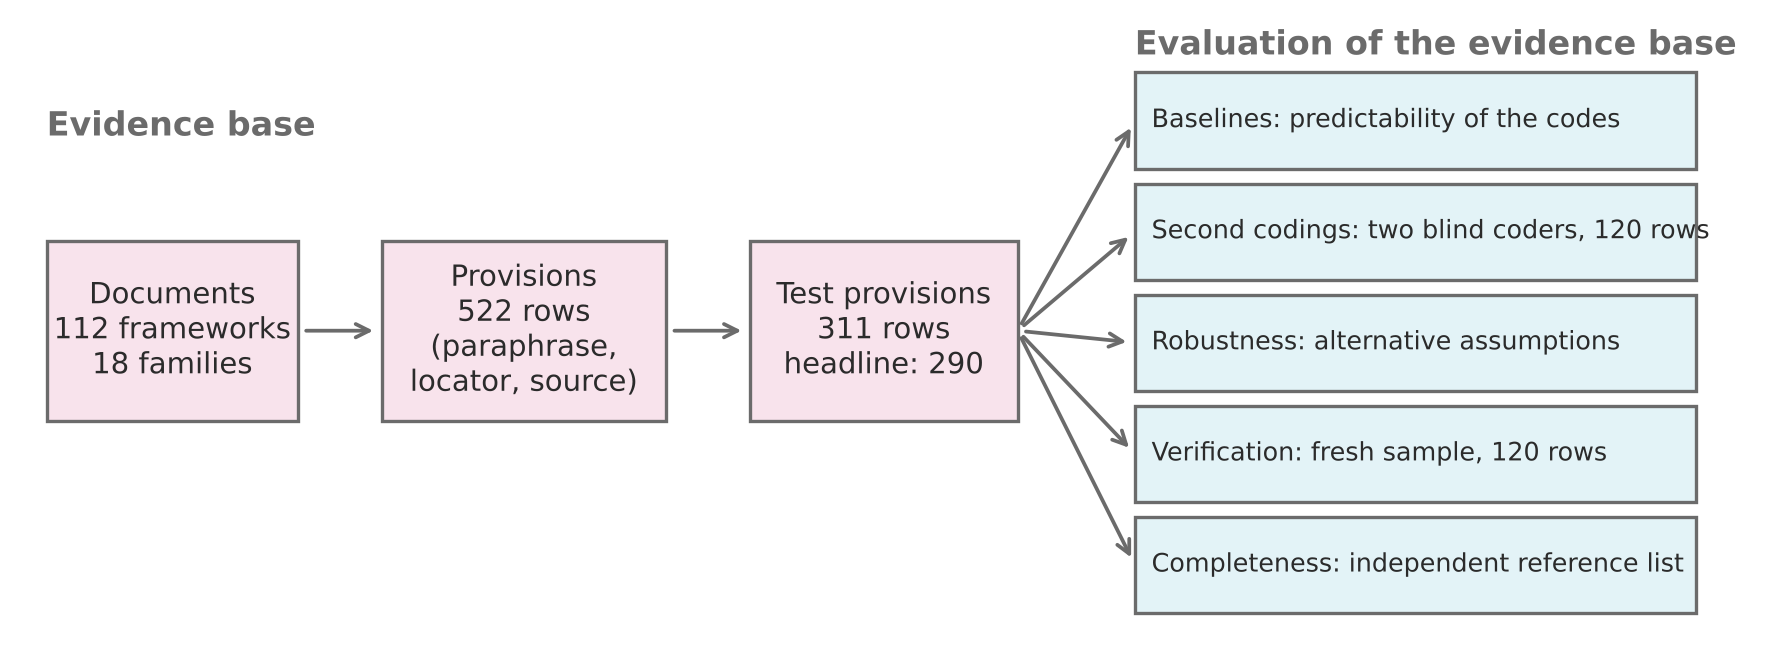
\includegraphics[width=0.96\linewidth]{figures/fig1_pipeline.png}
\caption{Structure of the study. Provisions are extracted from primary documents into a table; the headline analysis uses test provisions that pass a verification screen; five checks evaluate the table.}\label{fig:pipeline}
\end{figure}

\paragraph{Research questions.} We ask: \textbf{RQ1} How much of what documents say about pre deployment testing is binding, and does this depend on the family of documents or the type of test? \textbf{RQ2} Do binding provisions say how to test, more than other provisions do? \textbf{RQ3} Can the codes be predicted from simpler signals, and which signal drives them? \textbf{RQ4} Do independent coders reproduce the codes? \textbf{RQ5} Does the headline finding survive reasonable changes to coding choices? \textbf{RQ6} How often does a row misstate its source, and how much of the relevant literature does the table miss? \textbf{RQ7} Does a checklist tool built on the table behave correctly against a specification written before the tool was run?

\paragraph{Contributions.} (1) A clause level evidence table with binding force, test type, source locator, retrieval date and verification status per row (Section~\ref{sec:method}). (2) A measured answer to RQ1 and RQ2, including a four level specificity coding of every headline row (Section~\ref{sec:findings}). (3) An audit protocol with baselines, blind second codings, robustness analysis, a fresh verification sample and a completeness pilot, with its results and its failures reported (Section~\ref{sec:audit}). (4) A three valued checklist tool and its evaluation against preregistered scenarios (Section~\ref{sec:tool}). (5) A traceability map from every number in the paper to a committed result file (Appendix~\ref{app:trace}). This is research analysis and not legal advice.

\section{Related work}
\paragraph{Comparative studies and datasets of AI governance.} Comparisons of AI regulation across jurisdictions exist, for example of the European Union, the United States and China \citep{chun2024comparative,du2025toward}, a seven category framework applied to five jurisdictions \citep{roberts2023comparative}, and a comparison of risk classification and enforcement \citep{almaamari2025between}. The AI Governance and Regulatory Archive provides an annotated dataset of AI laws and policies, tagged at segment level with a taxonomy of risks, harms, governance strategies and application domains \citep{arnold2024agora}; it does not code binding force or test type. A computational study of 1,065 strategy and legislation documents measures hedging language across 64 countries \citep{silva2024decoding}, which is a document level use of wording cues for force. Cross document comparisons of company frontier safety policies find nine shared components, among them capability thresholds and evaluation timing \citep{metr2025common}, and score twelve such frameworks against 65 criteria \citep{stelling2025evaluating}; a mapping of company practice to a draft code of practice is related \citep{stelling2025mapping}. These cover voluntary company commitments. We narrow the question to one activity, testing before deployment, and record the force of each provision at clause level across governments, institutes and standards bodies. We found no work that codes binding force of AI governance clauses, which is a limit of a search run under a restricted budget and not a claim that none exists.

\paragraph{Audit, evaluation and assurance.} Internal auditing across the development lifecycle was proposed as a complement to external audits \citep{raji2020closing}; auditing at the level of providers, models and applications was proposed for language models \citep{mokander2023auditing}; black box access was argued to be insufficient \citep{casper2024blackbox}; third party audit ecosystems in finance, environment and health were compared \citep{raji2022outsider}; and a landscape analysis of 390 audit tools with interviews of 35 practitioners found thin support for harm discovery and audit communication \citep{ojewale2024towards}. Evaluation methods include holistic benchmarks \citep{liang2023holistic}, evaluations for dangerous capabilities \citep{shevlane2023model,phuong2024evaluating}, automated red teaming \citep{perez2022red} and a sociotechnical view of safety evaluation \citep{weidinger2023sociotechnical}; industry red teaming practices vary widely \citep{feffer2024red}, safety evaluations of generative systems leave gaps in coverage \citep{rauh2024gaps}, and benchmark quality is uneven \citep{reuel2024betterbench,bean2025measuring}. An evaluation science for generative systems is argued to be still under construction \citep{weidinger2025toward}. These works describe how to test and how well tests are done. We ask where documents say that testing must, should or does occur, which matters because a clause that says ``test'' does not fix the quality of the test.

\paragraph{The European Union Act and standards.} The force and mechanism of conformity assessment and post market monitoring have been analysed \citep{mokander2021conformity}, harmonised standards examined \citep{gornet2024european}, and reliance on self certification criticised \citep{wachter2024limitations}; two analyses concern the 2021 proposal \citep{mokander2021conformity,veale2021demystifying}, while our table uses the amended text of 2026. The Act is described as a framework for regulatory learning whose compliance leans on harmonised and international standards \citep{lewis2025mapping}, and attempts to translate its requirements into technical requirements find that some lack usable technical definitions \citep{guldimann2024complai}. Our table is consistent with the view that the Act leaves much to the provider but covers it as one family among sixteen. Voluntary testing frameworks such as that of Singapore \citep{lee2023aiverify,harjani2025singapore} and the NIST framework \citep{tabassi2023airmf} are guidance that organisations may adopt, and NIST has outlined a standard for testing, evaluation, verification and validation \citep{nist2025tevv}.

\paragraph{The Gulf and the public sector.} A document analysis of the six national AI strategies of the Gulf Cooperation Council finds reliance on soft regulation through strategies and ethical principles, with no comprehensive AI specific legislation at the time of its analysis \citep{albous2025gcc}; a legal overview describes non binding ethics guidelines and a non binding charter for the UAE \citep{hofverberg2024falqs}; a comparison of the UAE and Kuwait studies institutional mechanisms in public sector adoption and recommends pre deployment testing and audits without comparing existing requirements \citep{albous2025kuwaituae}. Evaluation of Arabic language models is described as uneven across dialects and benchmarks \citep{alzubaidi2025evaluating}, and safety evaluation concentrates on a few languages \citep{peppin2025multilingual}. We found no study of testing requirements for AI in the UAE or the Gulf. For the public sector, impact assessment frameworks were proposed early \citep{reisman2018aia} and cautioned against convenient metrics \citep{metcalf2021aias}; a framework for supreme audit institutions covers the lifecycle \citep{brand2025sai}; a national audit office found that few of nine government algorithms met its requirements \citep{rekenkamer2022audit9}; fears of bureaucratic burden were reported for a transparency standard in policing \citep{zilka2023police}; and a government roadmap plans an assurance market \citep{dsit2025assurance}. None compares pre deployment testing requirements across regulators.

\paragraph{Legal text classification and language models as coders.} Classifying obligation, permission and prohibition in legal text is an established task \citep{oneill2017classifying,sleimi2020semantic,ariai2024legalsurvey}. On 200 provisions of European Union regulation annotated by three people with six deontic classes, a small model beat a fine tuned legal language model on macro F1 while rare classes went unrecognised \citep{minkova2023lowresource}; for sentences containing shall or must in about 120,000 European legal acts, modal words alone did not settle whether a sentence regulates \citep{brandsma2025regulatory}; and requirements engineering studies compare language models with simple baselines on regulatory provisions \citep{hassani2025foodsafety}. Our binding status coding adds classes for non binding recommendation and for ambiguous force, which these studies do not model. Requirement levels such as MUST, SHOULD and MAY have formal definitions in some standards \citep{bradner1997key}, but conventions differ between document families, which motivates our wording rule baseline and its limits. Language models are increasingly used for annotation, with results from agreement above crowd workers \citep{gilardi2023chatgpt,tornberg2023chatgpt} to reliability that varies with prompt wording \citep{reiss2023testing}, performance on a par with the better law student annotators on legal concepts when guidelines are supplied \citep{savelka2023can}, and a requirement of validation against human labels \citep{pangakis2023automated}; surveys and benchmarks cover the practice \citep{tan2024large,ziems2024can}. Models are also used to extract rules from the AI Act, with checking that is itself model based \citep{guliani2026dejure}, and to judge compliance with expert labels of only moderate agreement \citep{marino2025airegbench}. In evidence synthesis, a study within reviews found error rates of 9.0\% for model assisted and 11.0\% for human only data extraction \citep{gartlehner2025swar}, and a joint position statement requires human oversight and reporting of model use \citep{flemyng2025position,gallifant2024tripodllm}. Because our coding was assisted by a language model, these results motivate blind second codings and a verification audit. Models fabricate references \citep{fabrication2023chatgpt,chelli2024hallucination,athaluri2023exploring,naser2026cite}, a risk for any table built with model assistance.

\paragraph{Agreement, completeness and preregistration.} Agreement is reported with Cohen's kappa \citep{mchugh2012interrater} and Krippendorff's alpha \citep{krippendorff2011computing}; kappa depends on the marginal distribution of labels \citep{wongpakaran2013comparison} and sample size requirements for kappa tests depend on it too \citep{bujang2017guidelines}, so we report percentage agreement beside kappa. Capture recapture methods have been used to estimate what a literature search misses \citep{spoor1996use,kastner2009capture,stelfox2013capture}, with doubts about duplicate identification \citep{motschall2009number}, and sampling based estimators of residual relevant documents exist for ranked review \citep{li2020stop}; our completeness check is a simpler pilot against an independent reference list. Preregistration separates prediction from postdiction \citep{nosek2018preregistration}, templates exist for NLP research and predictive modelling \citep{vanmiltenburg2021preregistering,hofman2023preregistration}, and datasheets document datasets \citep{gebru2021datasheets}. We state which parts of our protocol were committed before they were run and which were not.

\section{Evidence base and method}\label{sec:method}
\subsection{Frame, rows and coding}
We included primary documents from governments, national institutes and standards bodies that were retrieved and read and that contain at least one provision on testing, evaluation, assessment, validation, conformity, red teaming, audit or verification of an AI system before or at deployment. Secondary sources were used only to locate primary ones. Each provision is a row with the clause or page, a paraphrase, the source address, the retrieval date, a binding status and a verification status. Of 522 rows, 311 are test provisions (a provision that calls for, or describes as practice, an evaluation that produces evidence), 122 are enablers such as documentation or logging, and 89 are context such as dates and penalties.

Binding status has five values. \emph{Mandatory} means binding on the stated actor with the duty in operative text. \emph{Conditional} means binding only if a trigger applies, such as a risk class. \emph{Voluntary} is a formal scheme or standard an organisation may adopt. \emph{Guidance} is a recommendation or a description of practice. \emph{Ambiguous} is used where the force of the source cannot be settled from the text. Each test row also has a primary test type from a taxonomy of fifteen types (Appendix~\ref{app:taxonomy}). The headline analysis uses the 290 test rows that are not unverified, unverifiable or dependent on a portal summary; 21 test rows are excluded for these reasons, and their effect is bounded in Section~\ref{sec:robust}. Coding is judgemental and was assisted by language model agents (Section~\ref{sec:ethics} and Appendix~\ref{app:llm}).

\subsection{Access rule}
Only standard fetch and search tools were used. If a site rejected a fetch, the attempt was recorded and no workaround was used (no changed user agent, cache, mirror or third party copy). The row is then marked unverified because the source was blocked, excluded from the headline, and the document is listed for a person to download. 32 rows (of all types) were blocked in this way. Two further kinds of row rest on weaker access: 89 rows were read from an English translation or a machine rendering of the original, and 19 rows (12 of them headline rows) come from ISO catalogue pages, where the paywalled standard text was not read. Each row records which applies.

\subsection{Corpus}
Table~\ref{tab:family} gives the headline rows by family. Families differ greatly in size, and the table is not a sample of a defined population: documents were chosen because they mention testing and because they could be retrieved, which is why completeness is estimated separately (Section~\ref{sec:complete}).

\begin{table}[t]\centering\small
\begin{tabular}{lrrrrrr}
\toprule
Family & Docs & Rows & Binding & Vol./guid. & Ambig. & Binding \% (95\% CI) \\
\midrule
US-OMB & 1 & 3 & 3 & 0 & 0 & 100 (44 to 100) \\
EU-AI-Act & 3 & 31 & 27 & 4 & 0 & 87 (71 to 95) \\
UAE-AbuDhabi-DoH & 3 & 17 & 11 & 0 & 6 & 65 (41 to 83) \\
China & 7 & 17 & 10 & 7 & 0 & 59 (36 to 78) \\
Korea & 2 & 6 & 3 & 3 & 0 & 50 (19 to 81) \\
UAE-DIFC-ADGM & 7 & 16 & 8 & 4 & 4 & 50 (28 to 72) \\
UAE-Federal & 7 & 22 & 9 & 12 & 1 & 41 (23 to 61) \\
UAE-Dubai & 6 & 20 & 7 & 12 & 1 & 35 (18 to 57) \\
Japan & 7 & 15 & 2 & 13 & 0 & 13 (4 to 38) \\
UK & 6 & 22 & 1 & 18 & 3 & 5 (1 to 22) \\
EU-GPAI-CoP & 1 & 9 & 0 & 9 & 0 & 0 (0 to 30) \\
EU-Standards & 1 & 1 & 0 & 1 & 0 & 0 (0 to 79) \\
ISO-IEC & 1 & 12 & 0 & 12 & 0 & 0 (0 to 24) \\
Saudi & 6 & 30 & 0 & 11 & 19 & 0 (0 to 11) \\
Singapore & 8 & 33 & 0 & 32 & 1 & 0 (0 to 10) \\
US-NIST & 5 & 36 & 0 & 36 & 0 & 0 (0 to 10) \\
All headline rows & 71 & 290 & 81 & 174 & 35 & 28 (23 to 33) \\
\bottomrule
\end{tabular}
\caption{Headline test provisions by family: number of documents with headline rows, rows by binding status, and the binding (mandatory or conditional) share with a 95\% Wilson interval over rows. Intervals ignore clustering by document and are narrow for that reason.}\label{tab:family}
\end{table}

\section{What the evidence says}\label{sec:findings}
\paragraph{RQ1: binding provisions are a minority.} Of 290 headline test provisions, 81 (28\%) are mandatory or conditional, 174 (60\%) are voluntary or guidance and 35 (12\%) are ambiguous. Figure~\ref{fig:family} shows that binding text is concentrated: the European Union Act supplies most of it, followed by Abu Dhabi health regulation, China, Korea, the DIFC and ADGM, and the single United States OMB memorandum, while the NIST, Singapore, ISO and general purpose model code families are almost entirely voluntary or guidance. 10 of 16 families contain any binding test provision, and 21 of 71 documents do.

\begin{figure}[t]\centering
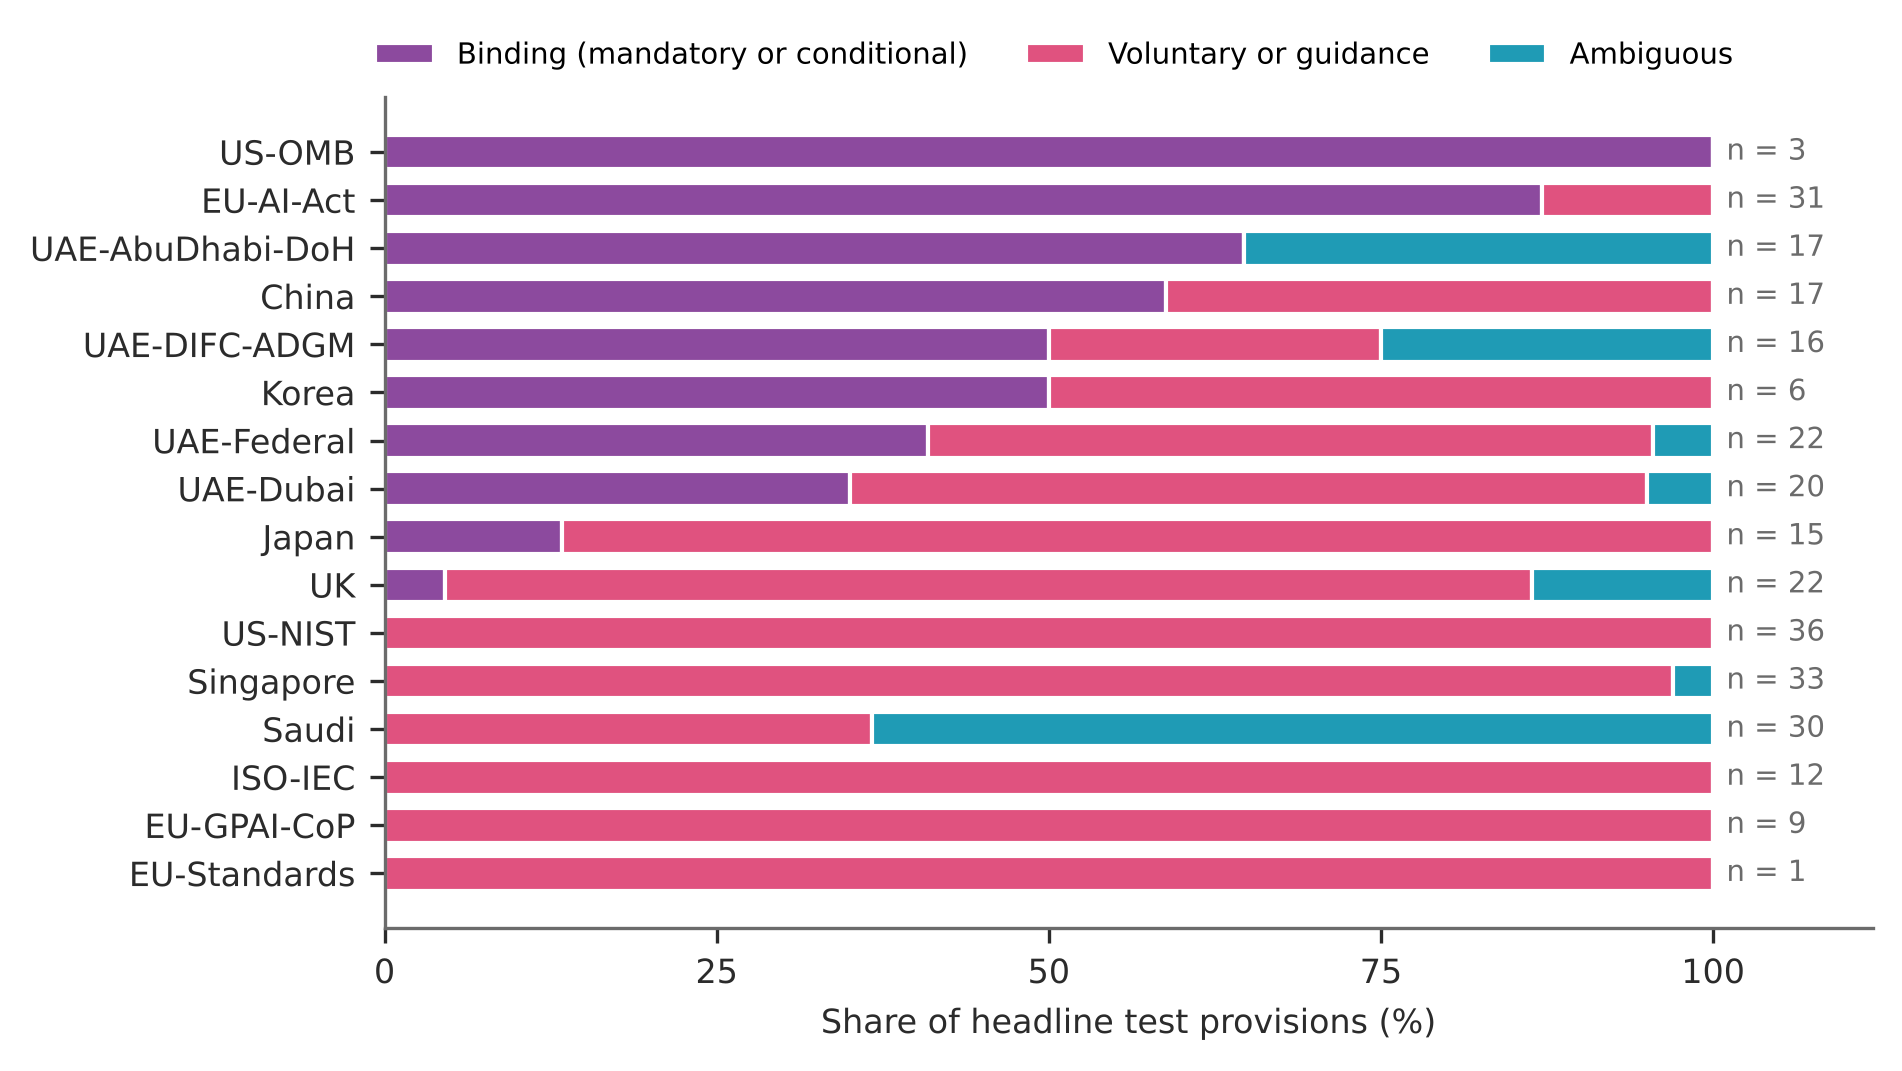
\includegraphics[width=0.86\linewidth]{figures/fig2_family.png}
\caption{Share of headline test provisions by binding status, for each family (families ordered by binding share; n is the number of rows).}\label{fig:family}
\end{figure}

\paragraph{Some test types are rarely binding.} Table~\ref{tab:types} gives the same counts by primary test type. Conformity assessment and risk or impact assessment have the largest binding counts, which is expected since these are the procedural duties of regulation. Of 26 headline rows coded red teaming or dangerous capability evaluation, 4 are binding. Human oversight validation has 1 headline row and content safety evaluation has 3; these counts are too small for more than a note. Shares differ by type, so they should not be ranked without the number of rows behind each.

\begin{table}[t]\centering\small
\begin{tabular}{llrrrr}
\toprule
Code & Test type & Rows & Binding & Vol./guid. & Ambig. \\
\midrule
PERF & Performance and validity & 58 & 7 & 47 & 4 \\
ROB & Robustness and reliability & 18 & 2 & 13 & 3 \\
FAIR & Fairness and representativeness & 18 & 3 & 13 & 2 \\
SEC & Security and adversarial resilience & 22 & 6 & 15 & 1 \\
RED & Red teaming and dangerous capability evaluation & 26 & 4 & 22 & 0 \\
CSAFE & Content safety evaluation & 3 & 0 & 3 & 0 \\
PRIV & Privacy and data protection assessment & 10 & 5 & 4 & 1 \\
TRANS & Transparency, explainability and reproducibility & 4 & 1 & 3 & 0 \\
OVER & Human oversight validation & 1 & 0 & 1 & 0 \\
RISK & Risk, impact and compliance assessment & 42 & 16 & 18 & 8 \\
DATA & Data quality validation & 6 & 3 & 2 & 1 \\
CONF & Conformity assessment, independent review, certification & 36 & 22 & 7 & 7 \\
REAL & Real world, sandbox and pilot testing & 8 & 1 & 5 & 2 \\
MON & Post deployment monitoring and re assessment & 18 & 6 & 10 & 2 \\
GATE & Acceptance criteria and release decision & 20 & 5 & 11 & 4 \\
\bottomrule
\end{tabular}
\caption{Headline test provisions by primary test type and binding status (mandatory or conditional counted as binding).}\label{tab:types}
\end{table}

\paragraph{Required, recommended and described.} Among 209 headline test rows that are not binding, two coders separated 19 that use obligation wording inside a non binding document, 140 that recommend a test and 40 that only describe practice; 10 were disputed. The distinction matters because a reader who sees ``shall'' in a guidance document may take it for a requirement.

\paragraph{RQ2: binding provisions are not more specific.} A common reading is that binding text requires that testing happens and is documented while leaving the metrics and thresholds to the provider. We tested this on all 290 headline rows. Two blind coders (language model instances that saw only the framework name, locator and paraphrase, not the binding status) assigned one of four levels: S1 process only, S2 property named, S3 method or metric named, S4 criterion set (Appendix~\ref{app:spec}). The coders agree on 87.9\% of rows and within one level on 97.2\% (kappa 0.827, 95\% interval 0.77 to 0.878; linear weighted 0.843). Figure~\ref{fig:spec} gives the distribution. Binding provisions are more often process only (24.7\% and 30.9\% by the two coders, against 7.5\% and 11.5\% for voluntary and guidance rows; difference 17.2 and 19.4 points, document level 95\% intervals 5.3 to 27.2 and 9.6 to 30.8). They are not more likely to name a method, metric or criterion (48.1\% and 39.5\% against 53.4\% and 48.3\%; intervals -19.8 to 10.3 and -22.2 to 6.6 include zero) or to set a criterion (13.6\% and 11.1\% against 9.2\% and 7.5\%). So the simple statement that binding text seldom says how is too strong: about 39.5\% to 48.1\% of binding rows name a method, metric or criterion, but they do so no more often than guidance does, and a larger share of them says only that testing occurs. The coding rests on the analyst's paraphrase, not on the source text, and both coders are models, so this is a measurement of the table and not of the sources.

\begin{figure}[t]\centering
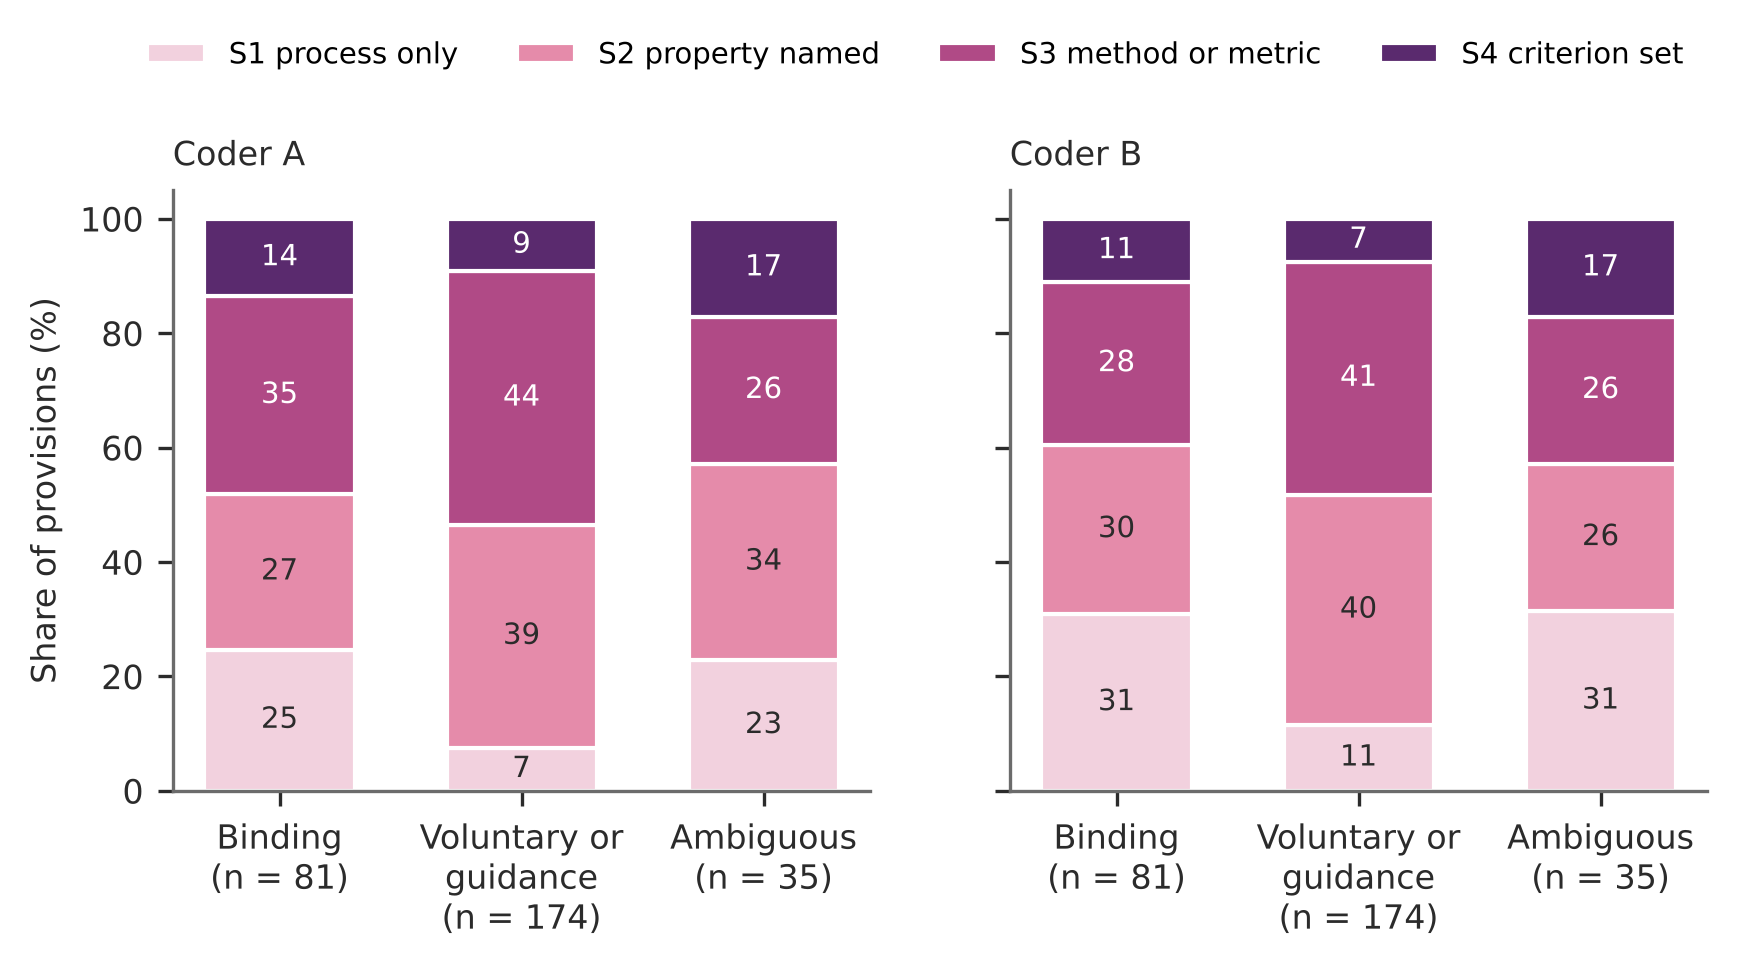
\includegraphics[width=0.92\linewidth]{figures/fig3_specificity.png}
\caption{Specificity of headline test provisions by binding status, as coded blind by two coders. Labels show percentages; segments below 5\% are unlabelled.}\label{fig:spec}
\end{figure}

\paragraph{UAE public sector.} We report what the retrieved sources contain and make no claim about what the UAE requires beyond them. One cross sector instrument that uses obligation wording for government entities, the national cyber security policy for AI, concerns AI security. Its scope over emirate level government entities was read differently by two verifiers, and its explicit before deployment wording sits in implementation guidance phrased as should. Other binding UAE testing text in the table is sector or zone specific (Abu Dhabi health, Dubai health, DIFC Regulation 10). We found no UAE federal technical standard for functional, fairness or accuracy testing of AI in government. Several instruments, among them a central bank guidance note, could not be read, and some may not be public. Absence in this table is not evidence of absence in law.

\section{Auditing the evidence base}\label{sec:audit}
\subsection{Baselines (RQ3)}\label{sec:baselines}
We ask how well the two main codings can be predicted by methods much simpler than reading the document, using the 290 headline rows. Methods were chosen by the analyst, who had seen the table, and committed with the code: a majority class; a document prior (the most common label among training rows of the same document); a wording rule for binding status (obligation words against recommendation words) and a keyword rule for test type built from the taxonomy definitions; TF-IDF with logistic regression; and a frozen sentence embedding (all-MiniLM-L6-v2, no fine tuning) with logistic regression whose regularisation is chosen by inner cross validation. The last two are also given a document indicator. Protocols are 10 times repeated stratified five fold cross validation (CV) and leave one family out (LOFO), which removes every document of a family from training. Table~\ref{tab:bl} and Figure~\ref{fig:bl} give accuracy; macro F1 and intervals are in the repository.

\begin{table}[t]\centering\small
\begin{tabular}{lrrrrr}
\toprule
Method & Binding (5) CV & Binding (5) LOFO & Binding (3) CV & Type CV & Type LOFO \\
\midrule
Majority class & 45.5 & 45.5 & 60.0 & 20.0 & 14.5 \\
Document prior & 84.3 & 45.5 & 89.6 & 27.8 & 14.5 \\
Wording rule & 58.3 & 58.3 & 76.9 & n/a & n/a \\
Keyword rule & n/a & n/a & n/a & 47.2 & 47.2 \\
TF-IDF, logistic regression & 50.9 & 46.9 & 64.9 & 29.9 & 25.2 \\
TF-IDF plus document & 79.1 & 45.5 & 84.7 & 32.2 & 22.8 \\
Embedding, logistic regression & 61.7 & 49.3 & 73.5 & 61.2 & 53.8 \\
Embedding plus document & 82.9 & 47.9 & 88.0 & 55.0 & 51.4 \\
\bottomrule
\end{tabular}
\caption{Accuracy (\%) of baselines for binding status in five classes, binding status in three classes and primary test type. n/a means the method does not apply to that task.}\label{tab:bl}
\end{table}

\begin{figure}[t]\centering
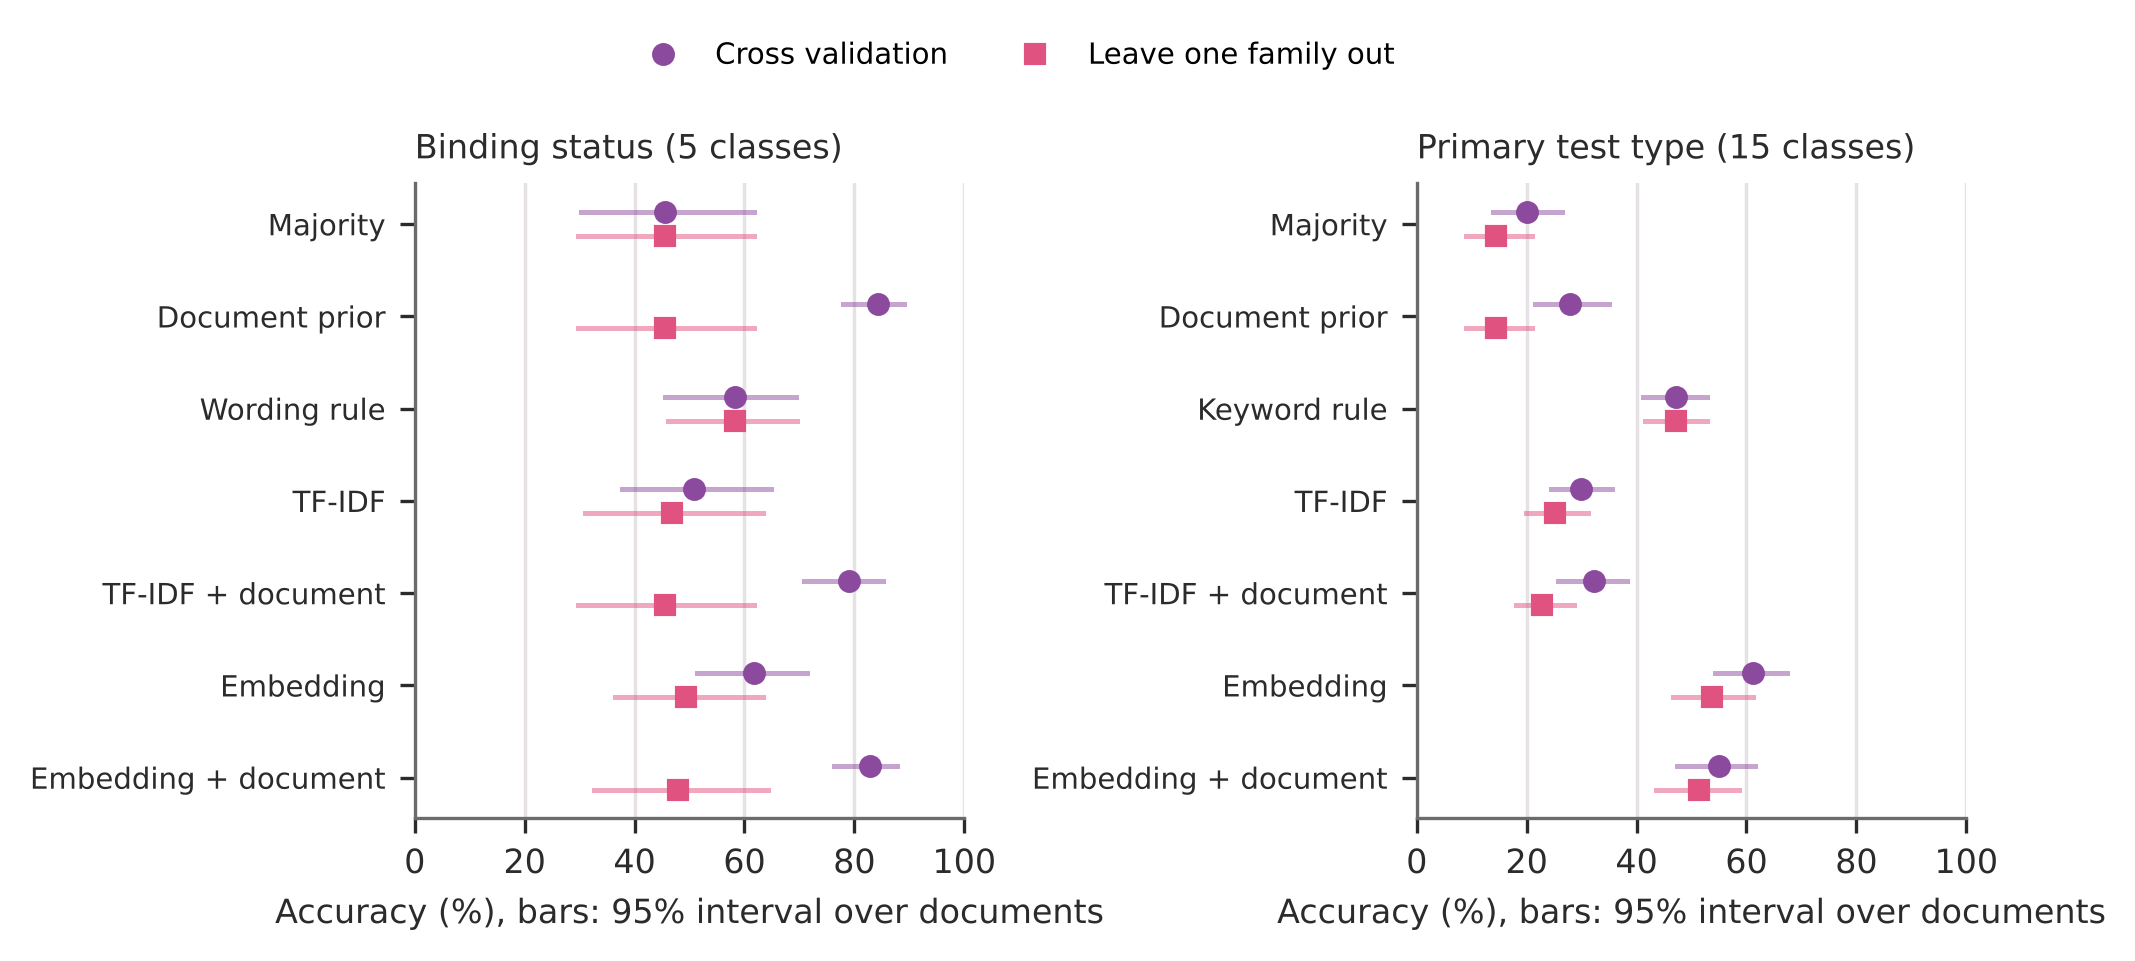
\includegraphics[width=\linewidth]{figures/fig4_baselines.png}
\caption{Accuracy of baselines under cross validation and leave one family out. Bars are 95\% intervals from a bootstrap over documents.}\label{fig:bl}
\end{figure}

Binding status is largely a property of the document: a document prior reaches 84.3\% when other provisions of the same document were seen in training, against 45.5\% for the majority class, and falls back to the majority rate under LOFO (45.5\%) because it has nothing to look up. This is close to tautological, since provisions of one document tend to share its force, but it shows how much of the signal is document identity. The wording of a single provision carries some information, since the wording rule beats the majority class (58.3\% against 45.5\%), and it is the only method above the majority class by a wide margin on held out families (58.3\%, against 49.3\% for the embedding and 46.9\% for TF-IDF), although document level intervals overlap heavily, so the ordering is suggestive and the learned models are not clearly better than the majority class on unseen families. For test type the picture reverses: the embedding (61.2\% under CV, 53.8\% under LOFO) beats the keyword rule (47.2\%), which beats TF-IDF (29.9\%) and the majority class (20.0\%); the test type is recoverable from the text of the paraphrase, binding status is not. These scores show that the coding is regular and not that it is correct, since the labels are the analyst's own and the paraphrase being classified was written by the same analyst. Intervals over rows ignore clustering by document (80.2 to 88.2 for the document prior) and the document level interval is wider (78.0 to 89.0); Figure~\ref{fig:bl} uses the latter. The keyword lexicon was written by an analyst who had seen the table. Any later classifier must beat the document prior and the wording rule, not only the majority class.

\subsection{Coding reliability (RQ4)}
Two coders who saw the row paraphrase, the document name and the locator, and a written codebook but not the original codes, recoded 120 randomly chosen headline rows. Table~\ref{tab:ag} gives percentage agreement and Cohen's kappa for each pair, and Krippendorff's alpha over three coders.

\begin{table}[t]\centering\small
\begin{tabular}{lrrrr}
\toprule
Field & Orig.\ and B2 & Orig.\ and B3 & B2 and B3 & Alpha (3) \\
\midrule
Binding status (5) & 75.8 / 0.64 & 77.5 / 0.66 & 94.2 / 0.91 & 0.73 \\
Binding status (3) & 83.3 / 0.66 & 83.3 / 0.66 & 96.7 / 0.92 & 0.74 \\
Primary test type & 78.3 / 0.76 & 78.3 / 0.76 & 90.0 / 0.89 & 0.80 \\
\bottomrule
\end{tabular}
\caption{Agreement (percent / kappa) between the original coding and two blind coders (B2, B3), and alpha over the three.}\label{tab:ag}
\end{table}

The blind coders agree closely with each other (kappa 0.905 on five classes). Each agrees less with the original coding (kappa 0.636 to 0.662). Of the 30 five class disagreements where exactly one coder differs, the original is the odd one out in 24 (one further row has three different codes). The original coder used ambiguous on 20 of 120 rows, against 5 and 2 for the blind coders, and the commonest pattern is ambiguous in the original against guidance in both blind codings. Two things could produce this and we cannot separate them: the original coder read the whole document while the blind coders read one provision, and the written instructions differed (the blind codebook asks for ambiguous to be used sparingly). The choice of coder moves the headline only a little in this sample: the binding share is 21.7\% under the original coding and 23.3\% and 25.0\% under the blind codings, but the ambiguous share is 16.7\% against 4.2\% and 1.7\%, so the split between non binding and ambiguous depends on the coder. Because the coders saw the analyst's paraphrase and the document name, agreement is probably higher than it would be on raw text; agreement among coders is not accuracy; and all three coders are language models, so errors may be correlated. A human second coding of 100 rows is prepared and is the planned remedy.

\subsection{Robustness of the headline (RQ5)}\label{sec:robust}
Table~\ref{tab:rb} and Figure~\ref{fig:rb} recompute the binding share of test provisions under changes that a sceptical reader might propose: dropping each family in turn, adding back the 21 excluded test rows as all binding, counting every ambiguous row as binding, doing both, weighting each document equally, and resampling documents.

\begin{table}[t]\centering\small
\begin{tabular}{lr}
\toprule
Scenario & Binding share (\%) \\
\midrule
Headline test rows as coded & 27.9 \\
Leave one family out, range & 20.8 to 31.9 \\
Excluded rows added back, all binding & 32.8 \\
Ambiguous rows all binding & 40.0 \\
Both, most favourable to binding & 44.1 \\
Each document weighted equally & 25.5 \\
Document level bootstrap, 95\% interval & 13.4 to 43.7 \\
\bottomrule
\end{tabular}
\caption{Binding (mandatory or conditional) share of test provisions under alternative assumptions.}\label{tab:rb}
\end{table}

\begin{figure}[t]\centering
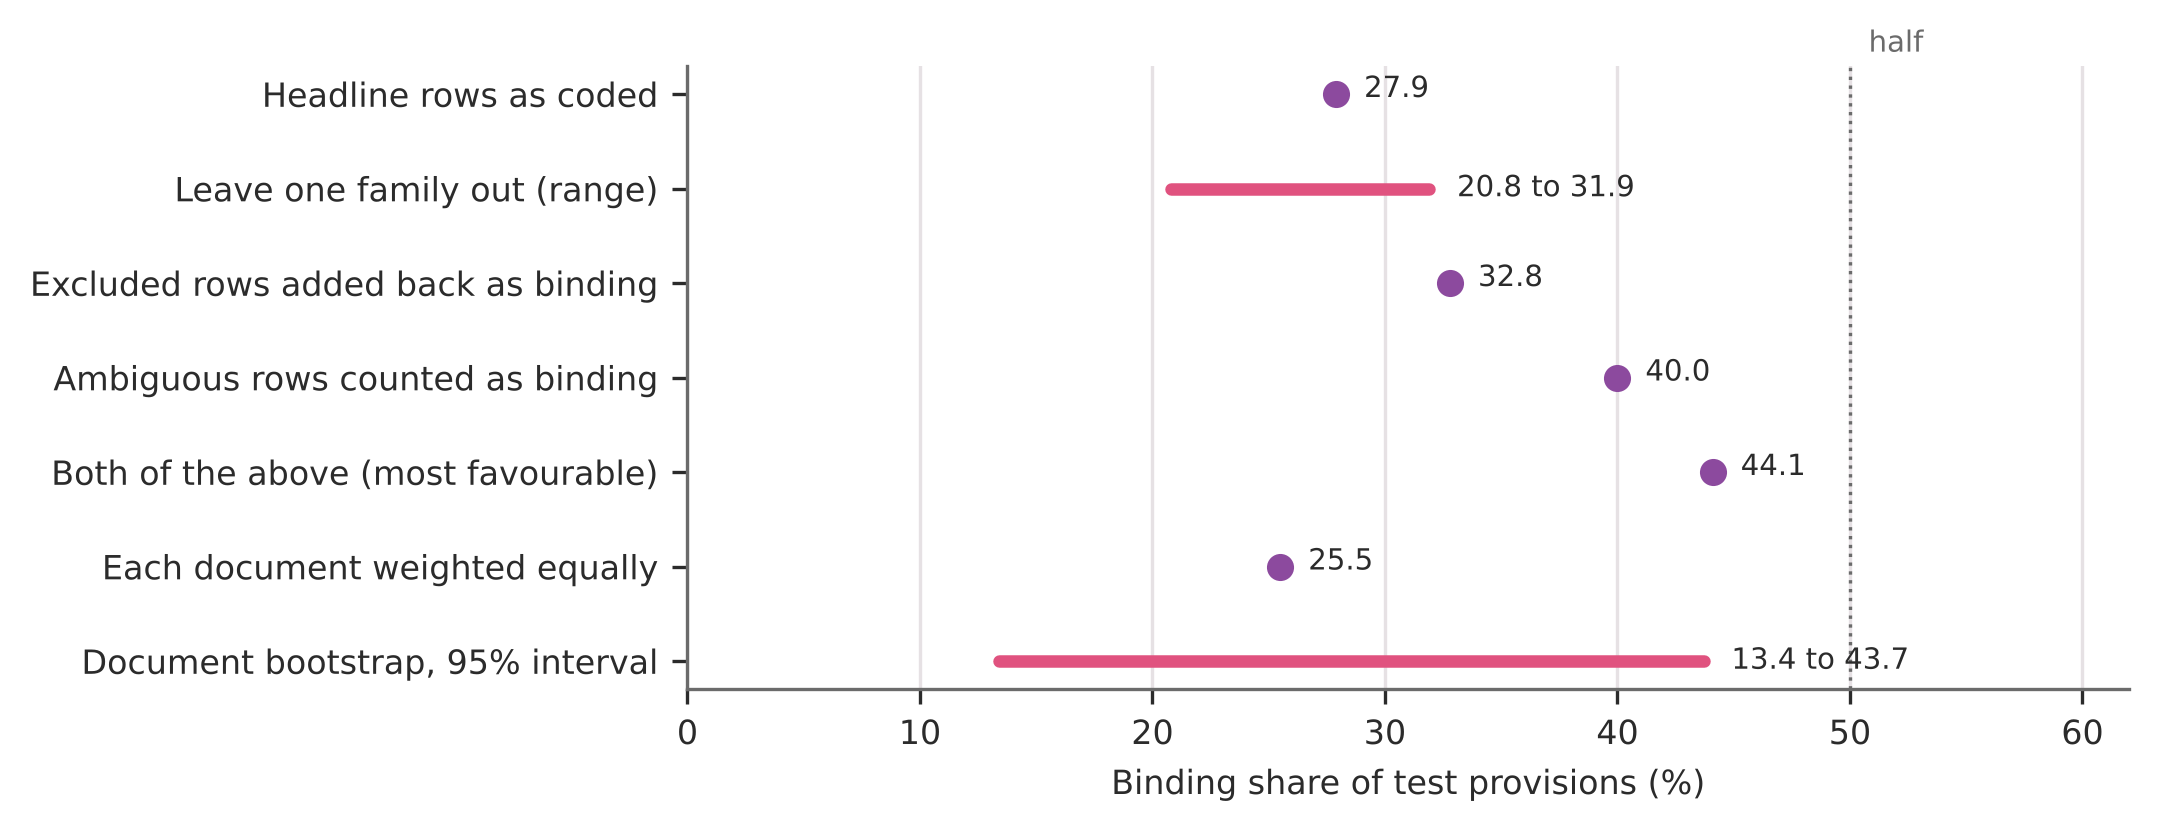
\includegraphics[width=0.9\linewidth]{figures/fig5_robustness.png}
\caption{Binding share under alternative assumptions. The most favourable combination stays below half.}\label{fig:rb}
\end{figure}

The statement that binding provisions are a minority survives every scenario we tried. The most favourable combination gives 44.1\%. Leaving out one family at a time gives 20.8\% to 31.9\%, weighting each document equally gives 25.5\% and weighting each family equally gives 31.5\%. The document level interval (13.4 to 43.7) is wide, so the size of the minority depends on coding and sampling choices and should be quoted with its range.

\subsection{Fresh independent verification (RQ6)}\label{sec:verify}
We drew 120 rows at random with a fixed seed from the 485 rows that earlier checks had marked verified, and independent verifiers saw only the row and the rules and reread the primary source. Of these, 94 could be read in the working session and 26 could not (21.7\%), mostly because of a session level domain restriction and not because sites refused. Table~\ref{tab:vf} gives the error rates on readable rows. After strict grading 6 rows had an error; they are listed in Appendix~\ref{app:errors} and accepted corrections were applied to the table. If every unreadable row were an error, the rate for the whole sample would be as high as 26.7\%, so we report the rate for readable rows. This rate is for rows that earlier checks had already passed and for the readable part of the sample: only 17 of 26 sampled European Union rows could be read, and that family supplies a large share of the binding rows, so the rate says little about them. The earlier phase 3 fresh sample, drawn before the corrections, found 3 errors in 23 verifiable rows (13.0\%, 95\% interval 4.5 to 32.1), and a recheck of rows left open found 15 in 142 (10.6\%). The samples are reported separately because they were drawn at different times. The true error rate of the whole table is plausibly higher than the readable subset suggests, and all verifiers are language models.

\begin{table}[t]\centering\small
\begin{tabular}{lrrr}
\toprule
Measure & Rows & Rate (\%) & 95\% interval \\
\midrule
Errors as graded by the verifier & 4 of 94 & 4.3 & 1.7 to 10.4 \\
Errors after strict grading & 6 of 94 & 6.4 & 3.0 to 13.2 \\
Any fault, including minor & 20 of 94 & 21.3 & 14.2 to 30.6 \\
\bottomrule
\end{tabular}
\caption{Fresh verification sample, readable rows only.}\label{tab:vf}
\end{table}

\subsection{Completeness pilot (RQ6)}\label{sec:complete}
A separate agent built a reference list of 82 candidate documents without seeing the table, and matches were made by hand. Of 19 candidates confirmed to contain a testing provision, 13 are in the table, a recall of 68.4\% (95\% interval 46.0 to 84.6); a further 58 candidates could not be resolved either way, and counting all of them as misses gives a lower bound of 55.8\%. The confirmed misses are all documents of the United States federal government (NIST, OMB and the national action plan); all 6 were read afterwards and 19 candidate rows drafted, which are held out of the table and unverified so that they do not inflate recall by construction. Of the 28 unresolved candidates that are not in the table, 6 are UAE instruments, which matters because the UAE is the application focus. Matching was done by hand by the author of the table. This is a pilot under the same tool limits as the table and is not a population estimate. The table should not be described as complete.

\section{The checklist tool (RQ7)}\label{sec:tool}
The tool turns the table into a list of 30 checklist items for an organisation. It reads answers to a small set of questions (system type, decision impact, entity zone, audience, data types, acquisition route, European market, hosting) and returns for each item APPLIES, DOES\_NOT\_APPLY or UNKNOWN, with the rows that support the item. Evaluation uses a Kleene three valued logic: a missing or unknown answer never makes a condition true or false. For each item the tool also says which answers would settle it. Whether a source binds the organisation is reported separately and is YES only when the answers settle that the organisation is the actor the source names.

\paragraph{Evaluation.} We wrote 94 scenarios from the checklist specification alone, with expected results from an independent oracle, and committed them before the engine was run: 82 with a specified result, 12 invalid inputs, ten stated assumptions and five monotone pairs. Table~\ref{tab:tool} compares the engine with four naive designs.

\begin{table}[t]\centering\small
\begin{tabular}{lrrrr}
\toprule
Method & Accuracy (\%) & Wrongly excluded & Wrongly applied & Unknown \\
\midrule
Three valued engine & 99.9 & 0 & 0 & 1062 \\
Two valued, missing counts as no & 56.8 & 1062 & 0 & 0 \\
Two valued, missing counts as yes & 57.0 & 45 & 1014 & 0 \\
Every item applies & 49.7 & 0 & 1238 & 0 \\
Answers ignored & 83.0 & 0 & 0 & 1476 \\
\bottomrule
\end{tabular}
\caption{Item level results over 82 specified scenarios (2460 decisions). Wrongly excluded: said not applicable where applicable or unknown was expected. Wrongly applied: said applicable where not applicable or unknown was expected.}\label{tab:tool}
\end{table}

The engine agreed on 2457 of 2460 decisions (99.9\%) and matched 81 of 82 scenarios exactly, and it never wrongly excluded or wrongly applied an item. The two valued designs score about 57\% because they cannot express unknown, and they are unsafe in opposite ways: the closed design drops items the user cannot yet rule out, and the open design applies items that do not apply. The fairer comparison is with the design that ignores the answers and returns unknown for conditional items (83.0\% with no errors), which the engine beats because it uses the answers; the oracle itself uses three valued logic, so two valued designs are penalised by construction. The scenarios were also used to find and fix two engine defects, so the figure for the final engine is after tuning, which is why the first run is reported. The first run, before any change, with the scenarios committed before the engine was run (commit order is the only timestamp), matched 2454 decisions, wrongly excluded 3 items (an empty list for a multiple choice question was treated as a known answer) and crashed on 3 of 12 invalid inputs (a list given for a single value question). These defects were fixed with tests and the scenarios rerun without editing the expectations. Of the 12 invalid inputs, 2 were accepted: a comma separated string for a multiple choice question is split into a list by design, which the preregistration had not expected. One scenario still disagrees: an unknown inside a list of values, where the oracle expected APPLIES and the engine conservatively returns UNKNOWN because the specification was ambiguous. A simulation of 3000 random profiles answered one question at a time found 0 flips between APPLIES and DOES\_NOT\_APPLY in 24000 steps. The scenarios test that the engine implements the checklist as written; they do not show that the checklist rules are legally correct.

\paragraph{Behaviour on synthetic deployment profiles.} To see whether the output differs sensibly between deployments we ran the tool on 8 invented profiles (Appendix~\ref{app:arch}). With no answers 18 of 30 items are unknown; with all eight questions answered between 0 and 3 remain (Figure~\ref{fig:arch}). 17 of 30 items change state between profiles and 12 apply to every profile. The tool reports a cited source as binding the organisation in only 1 of the 8 profiles (the Abu Dhabi health profile), because applicability rules are encoded for few instruments. This is deliberate and conservative, and it also shows that the tool cannot yet say which binding source applies to most organisations. A worked example for a synthetic, undeployed prototype, Madoun, is in the repository: 16 items apply, 2 do not and 12 remain unknown. No user study was done.

\begin{figure}[t]\centering
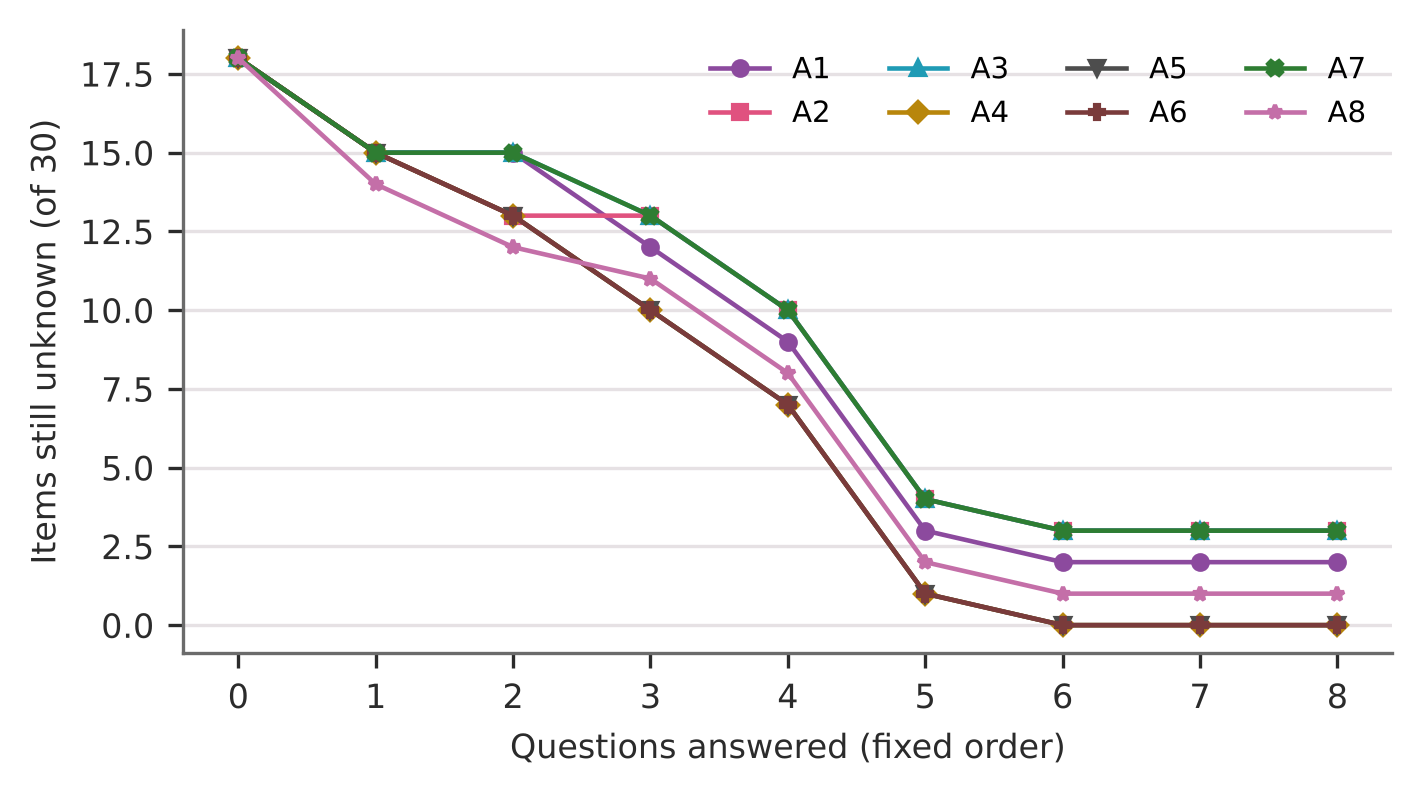
\includegraphics[width=0.62\linewidth]{figures/fig6_archetypes.png}
\caption{Items still unknown as questions are answered, for eight synthetic profiles (labels A1 to A8, Appendix~\ref{app:arch}).}\label{fig:arch}
\end{figure}

\section{Discussion}
\paragraph{What this means for a reader of the sources.} A reader who treats every mention of testing as a requirement is wrong about 60\% of the headline provisions and arguably about some of the 12\% that cannot be settled from the text. The practical rule that follows is to read the force of the document and the actor before the wording of the clause, since force is a property of the document and the wording of a single clause predicts it only moderately on unseen families (Section~\ref{sec:baselines}).

\paragraph{What this means for authors of requirements.} Binding provisions are no more specific than guidance, and a quarter or more of them say only that some testing happens. Where a regime leaves the metric to the provider or to a later standard, a reader cannot tell from the text whether a given test discharges the duty, and the research on benchmark validity suggests that the choice matters \citep{reuel2024betterbench,bean2025measuring}. Requirements that name a method, a data condition or a pass criterion, or that point to a standard that does, would be easier to meet and to audit. We state this as a consequence of the measurement and not as a finding about the intent of any regulator.

\paragraph{What this means for building evidence bases.} The audit shows how much a single analyst's table can hide. Binding status was reproduced by blind coders at kappa near 0.65 against the original and near 0.9 between blind coders, which indicates codebook sensitivity at the ambiguous boundary rather than random error; 6 of 94 readable sampled rows had a strict error; and about a quarter of a fresh sample could not be reread at all. We recommend that comparable tables report agreement against a blind recoding, a fresh verification sample with its unreadable share, and a completeness estimate, and release the coding inputs.

\section{Threats to validity and limitations}\label{sec:limits}
\begin{itemize}
\item \textbf{Coding by language model agents.} The original coding, second codings, specificity codings and verifications were produced by agents of the same family, so errors can be correlated. A human second coding and a domain or legal review have not been done. The bias this can introduce is not known in direction.
\item \textbf{Paraphrase circularity.} The blind coders and the baselines read the analyst's paraphrase, not the source text; agreement and predictability are therefore probably overstated as measures of fidelity to the source.
\item \textbf{Unread sources.} 32 rows come from sources that could not be read and are excluded from the headline, and 21.7\% of the fresh verification sample could not be read. Error rates describe readable rows, and the largest unreadable block is the European Union family.
\item \textbf{Completeness and selection.} The completeness pilot found a recall of 68.4\% on confirmed candidates, with an unresolved remainder. Documents were selected because they mention testing, so shares of binding provisions describe this sample and not all AI governance. Documents in languages other than English and non public instruments are under represented, and Arabic originals were read for a minority of UAE sources.
\item \textbf{Units of analysis.} A long guidance document yields many rows and a short statute few, so counts are not league tables. Intervals over rows ignore clustering; the document level analyses are wider.
\item \textbf{Currency.} Several documents were being revised at retrieval. Rows carry retrieval dates, and time sensitive items are listed in the repository.
\item \textbf{Tool.} Evaluation is against scenarios and synthetic profiles, with no user study. Applicability rules are the author's proposals and have not been reviewed by a lawyer.
\item \textbf{Literature.} The related work search ran under a restricted budget. Works cited were opened; 69 of 81 were read in full text and the rest at abstract or landing page level, as marked in the repository.
\item \textbf{Not legal advice.} Nothing here states what any law requires of any organisation.
\end{itemize}

\section{Ethics, AI assistance and availability}\label{sec:ethics}
The study uses public documents and involves no human subjects and no personal data. Research subagents built on a large language model searched for and read sources, extracted rows and proposed codes. Separate instances verified rows and made the second codings and the specificity codings. The author set the aims and the rules. The orchestrating agent regraded some verifier outputs against the rubric (14 in the third phase and two in the fourth); these calls are recorded in the decision log and a human review of them has not been done. Appendix~\ref{app:llm} lists the reporting items for model assisted work. Verification reduces but does not remove the risk of fabricated or misread content, and the sections above report the measured error rate. Data, code, tests and the decision log are available in the project repository (hudasol/ikhtibar), which records the licence terms of each part. Every number in this paper is read from a committed result file, and a test fails if a result file is older than the table it describes.

\section{Conclusion}
In this sample of documents, which were chosen because they mention testing, testing AI before deployment is mentioned far more often than it is required. Fewer than half of headline test provisions are binding under every assumption we tried, binding provisions are no more specific than guidance and more often say only that testing happens, and red teaming, content safety evaluation and human oversight validation have few binding provisions or none. The table is documented and partly independently checked, with a measured error rate and a measured gap in coverage. It is not complete and not error free. The next steps are a human second coding, a domain and legal review, rereading the blocked sources, and a larger completeness benchmark.

\bibliographystyle{plainnat}
\bibliography{refs}

\clearpage
\appendix
\section{Taxonomy of test types}\label{app:taxonomy}
\begin{tabular}{ll}
\toprule
Code & Test type \\
\midrule
PERF & Performance and validity \\
ROB & Robustness and reliability \\
FAIR & Fairness and representativeness \\
SEC & Security and adversarial resilience \\
RED & Red teaming and dangerous capability evaluation \\
CSAFE & Content safety evaluation \\
PRIV & Privacy and data protection assessment \\
TRANS & Transparency, explainability and reproducibility \\
OVER & Human oversight validation \\
RISK & Risk, impact and compliance assessment \\
DATA & Data quality validation \\
CONF & Conformity assessment, independent review, certification \\
REAL & Real world, sandbox and pilot testing \\
MON & Post deployment monitoring and re assessment \\
GATE & Acceptance criteria and release decision \\
\bottomrule
\end{tabular}

\section{Specificity coding}\label{app:spec}
Levels: S1 process only; S2 property or kind of test named; S3 method, metric, procedure, data condition, evaluator type or required report content named; S4 pass criterion, numeric threshold, fixed frequency or named external test. Coders saw the framework name, locator and paraphrase only. The full codebook is \path{data/coding/phase5/CODEBOOK_SPECIFICITY.md}.

\begin{table}[h]\centering\small
\begin{tabular}{llrrrrr}
\toprule
Coder & Binding status & S1 & S2 & S3 & S4 & n \\
\midrule
Coder A & Binding & 20 & 22 & 28 & 11 & 81 \\
Coder A & Voluntary or guidance & 13 & 68 & 77 & 16 & 174 \\
Coder A & Ambiguous & 8 & 12 & 9 & 6 & 35 \\
Coder B & Binding & 25 & 24 & 23 & 9 & 81 \\
Coder B & Voluntary or guidance & 20 & 70 & 71 & 13 & 174 \\
Coder B & Ambiguous & 11 & 9 & 9 & 6 & 35 \\
\bottomrule
\end{tabular}
\caption{Specificity levels (counts) by binding status for the two blind coders.}
\end{table}

\section{Verification errors}\label{app:errors}
Strict errors in the fresh verification sample (grading by the verifier, regraded against the rubric by the orchestrating agent; corrections accepted into the table unless stated).

\begin{tabular}{llll}
\toprule
Row & Family & Error type & As graded \\
\midrule
EU-AI-Act-004 & EU-AI-Act & other & error \\
Korea-002 & Korea & wrong status & error \\
Korea-003 & Korea & understated & minor \\
UAE-DIFC-ADGM-010 & UAE-DIFC-ADGM & understated & error \\
UK-004 & UK & wrong status & error \\
US-NIST-033 & US-NIST & other & minor \\
\bottomrule
\end{tabular}

\section{Synthetic deployment profiles}\label{app:arch}
\begin{table}[h]\centering\small
\begin{tabular}{lp{7.6cm}rrrr}
\toprule
Id & Profile & Appl. & Not & Unkn. & YES \\
\midrule
A1 & Internal document search assistant, federal entity & 18 & 10 & 2 & 0 \\
A2 & Public facing citizen chatbot, Dubai government & 23 & 4 & 3 & 0 \\
A3 & Clinical risk prediction model, Abu Dhabi health & 21 & 6 & 3 & 9 \\
A4 & Automated benefit eligibility decision, Abu Dhabi government & 24 & 6 & 0 & 0 \\
A5 & Face matching at a border checkpoint, federal entity & 25 & 5 & 0 & 0 \\
A6 & Credit scoring model offered in the European market, financial centre firm & 24 & 6 & 0 & 0 \\
A7 & Agent that takes actions on internal systems, Dubai government & 23 & 4 & 3 & 0 \\
A8 & Rules based eligibility calculator (no learned model), federal entity & 20 & 9 & 1 & 0 \\
\bottomrule
\end{tabular}
\caption{Items applying, not applying and unknown out of 30 when all eight questions are answered; YES is the number of cited rows for which the tool reports that the source binds the organisation.}
\end{table}

\section{Reporting of language model assistance}\label{app:llm}
\begin{itemize}
\item \textbf{Tasks:} searching and reading sources, extracting and paraphrasing provisions, proposing codes, verifying rows against sources, blind second coding, specificity coding, drafting of text and code.
\item \textbf{Human role:} the author set the aims, the rules (access rule, house style, free tools only) and reviewed the outputs; no human coded rows in the study to date.
\item \textbf{Model identity and version:} the model family was the same for all tasks; the exact model name and version were not recorded in the repository during coding and will be stated by the author in the camera ready disclosure.
\item \textbf{Prompts and codebooks:} codebooks, verifier rules and coding inputs are in \path{data/coding/}, \path{data/verification/} and \path{docs/PROTOCOL.md}; blind coders were told not to open other files or search the web.
\item \textbf{Validation:} blind second codings, a fresh random verification sample, a baseline comparison, and robustness analysis, with results in Section~\ref{sec:audit}.
\item \textbf{Known limitations:} coders share a model family; no human gold labels yet; orchestrator regrading not independently reviewed.
\end{itemize}

\section{Traceability map}\label{app:trace}
Every number in the paper is read from a committed result file by \path{scripts/build_paper.py} through \path{src/ikhtibar/eval_values.py}; \texttt{python -m ikhtibar.build\_all} regenerates all result files and documents, and the test suite fails if a result file is stale or the paper differs from its template.

\begin{table}[h]\centering\footnotesize
\begin{tabular}{p{2.9cm}p{5.0cm}p{5.0cm}}
\toprule
Content & Result file & Code \\
\midrule
Evidence table, family and type counts & \path{data/evidence_table.csv} & \path{src/ikhtibar/build_table.py} \\
Baselines (Tab.~\ref{tab:bl}, Fig.~\ref{fig:bl}) & \path{data/baselines/results.json} & \path{src/ikhtibar/baselines.py} \\
Agreement (Tab.~\ref{tab:ag}) & \path{data/coding/phase4/agreement.json} & \path{src/ikhtibar/coding_agreement.py} \\
Specificity (Fig.~\ref{fig:spec}) & \path{data/specificity.json} & \path{src/ikhtibar/specificity.py} \\
Robustness (Tab.~\ref{tab:rb}) & \path{data/robustness.json} & \path{src/ikhtibar/robustness.py} \\
Verification (Tab.~\ref{tab:vf}) & \path{data/verification/phase4/stats_p4.json} & \path{src/ikhtibar/verify4.py} \\
Completeness & \path{data/completeness/recall.json} & \path{src/ikhtibar/completeness.py} \\
Tool evaluation (Tab.~\ref{tab:tool}) & \path{data/evaluation/results.json} & \path{src/ikhtibar/evaluate_tool.py} \\
Synthetic profiles (Fig.~\ref{fig:arch}) & \path{data/evaluation/archetypes.json} & \path{src/ikhtibar/archetypes.py} \\
Figures & \path{paper/figures/} & \path{scripts/make_figures.py} \\
Citation claim checks & \path{data/paper/lit/claimcheck_1.csv} (and 2, 3) & \path{scripts/p5_merge_refs.py} \\
\bottomrule
\end{tabular}
\caption{Where each result in the paper comes from.}
\end{table}

\paragraph{Following one claim to its source.} A row such as the European Union Act row EU-AI-Act-004 is a line of \path{data/evidence_table.csv} carrying the clause locator, the paraphrase, the source address, the retrieval date, the binding status and the verification status; the verification sample files in \path{data/verification/phase4/} show that it was reread and found to attribute a date to a page that does not state it, and the accepted correction is in \path{data/verification/phase4/patches_p4.json}.

\section{Reproducibility checklist}
Code, data and tests are in the repository; random seeds are fixed and recorded in the result files; software versions are recorded in \path{requirements*.txt} and result metadata; the embedding model is a public model whose embeddings are cached with a hash of the input; preregistered scenarios are committed before the engine run (by commit order); the sources of every row are public addresses with retrieval dates; sources that could not be read are listed with their reason; licences for data and code are proposed in \path{docs/LICENSING.md} and are to be applied by the author before release.
\end{document}
